\documentclass[a4paper,reqno]{article}
\addtolength{\textwidth}{2cm} \addtolength{\hoffset}{-1cm}
\addtolength{\textheight}{2cm} \addtolength{\voffset}{-.5cm}
\usepackage{amssymb}
\usepackage{amsmath}
\usepackage{amsthm}
\usepackage{graphicx}
\usepackage{amsfonts}
\usepackage[usenames]{color}
\usepackage{hyperref}
\usepackage{mathtools}
\mathtoolsset{showonlyrefs}
\usepackage{hyperref}
\usepackage[utf8]{inputenc}
\usepackage{listings}
\usepackage{color}



\definecolor{gray}{RGB}{100,100,100}
\definecolor{basiccolor}{RGB}{0, 43, 54}
\definecolor{keywordscolor1}{RGB}{88, 110, 117}
\definecolor{keywordscolor2}{RGB}{101, 123, 131}
\definecolor{keywordscolor3}{RGB}{147, 161, 161}
\definecolor{identifiercolor}{RGB}{37, 116, 206}
\definecolor{commentscolor}{RGB}{91, 69, 0}
\definecolor{attributescolor}{RGB}{203, 75, 22}
\definecolor{numberscolor}{RGB}{147, 161, 161}
\definecolor{stringscolor}{RGB}{48, 145, 134}
\definecolor{backgroundcolor}{RGB}{255, 255,255}

% DEFINE LSTSET

\lstset{basicstyle = \color{basiccolor}\footnotesize\ttfamily,                   % the size of the fonts that are used for the code
  identifierstyle = \color{identifiercolor},
  commentstyle = \itshape\color{commentscolor},            % comment style
  keywordstyle = \bfseries\color{keywordscolor1},          % keyword style
  keywordstyle = {[2]\bfseries\color{keywordscolor2}},
  keywordstyle = {[3]\bfseries\color{keywordscolor3}},
  keywordstyle = {[4]\bfseries\color{attributescolor}},
  stringstyle = \color{stringscolor},                     % string literal style
  backgroundcolor = \color{backgroundcolor}}


\newcommand{\myenv}{(\raisebox{0pt}{\mygraphic{.6em}})}
\newcommand{\pa}{\hspace{0.5cm}}

\begin{document}

\title{Projet 2A : La chambre la moins froide}
\maketitle
\newpage

\setlength{\parindent}{1cm}
\part*{Introduction}
L'équation de la chaleur est une équation aux dérivées partielles 
parabolique, pour décrire le phénomène physique de conduction thermique, introduite initialement en 1811 par Jean Baptiste Joseph Fourier. Cette problématique de la diffusion de la chaleur est un enjeu industriel central vos à vis la gestion de l'énergie. A l'heure de la COP 21, elle n'a d'ailleurs jamais semblée autant d'actualité. \\
Comment maximiser la température d'une chambre en ne jouant que sur la géométrie de cette dernière ? Cette question qui peut surprendre de prime abord - car des dogmes architecturaux nous pousse naïvement à supposer, par définition, que toute chambre respectable se doit d'être rectangulaire - prend alors tout son sens.
Cette recherche se place indéniablement dans un vaste domaine d'étude, au confluent des mathématiques et de l'informatique: l'optimisation de forme. \\


% PARTIE 1 
\part{Mise en place de l'étude}
Notre étude sera réalisée en deux dimensions, dans le plan $\mathbb{R}^2$. Par ailleurs, une chambre sera modélisée par un polygone. Nous allons principalement nous intéresser aux pentagones (polygones à 5 côtés), cependant d'autres polygones seront également testés pour mener à bien ce travail. \\
Cette étude n'est rien d'autre qu'un problème d'optimisation. En effet, nous chercherons à maximiser le critère: température moyenne d'une pièce dans \textbf{son régime stationnaire}. \\ Pour fixer les notations, à l'avenir, la température à la position repérée par le vecteur $x$ de la chambre $\Omega$ au temps $t$ sera notée $u(x,t)$. De plus, la température moyenne de la pièce s'exprime facilement par  $ \frac {1}{|\Omega|}\int_{\Omega} u(x,t) dx $ ou $|\Omega|$ représente l'aire de la chambre.\\
Par ailleurs, nous considérerons que la température dans la pièce $\Omega$ est pilotée par l'équation aux dérivées partielles: 
\\
\begin{equation}
\frac{\partial u}{\partial t}(x,t) = \Delta u(x,t) + f(x,t)
\end{equation}
Il s'agit de l'équation de la chaleur usuelle dans laquelle les diverses constantes caractéristiques du phénomène ont été égalisé à 1. Par ailleurs, $f(x,t)$ est un terme de source permettant de préciser le profil thermique de la pièce.
Une des données clef de ce problème est de bien comprendre que dés lors que nous souhaitons classer des polygones (ou plus généralement des formes géométriques quelconques) il faut nécessairement que nous fixions des caractéristiques. En effet comment comparer la température moyenne de deux pièces si pour un même radiateur elles sont d'aires ou de nombre de cotés différents ? \\
Voici le cahier des charges retenus: \\
- le nombre de sommets du polygone est fixé égal à 5 dans l'étude principale, c'est à dire que nous travaillons sur des pentagones; \\
- l'aire des polygones est fixée égale à $|\Omega|$; \\
- toutes les chambres seront chauffées grâce à un même radiateur. Pour le modéliser, nous considérerons qu'un mur (c'est à dire un coté du polygone) de longueur fixée $l$ est sujet à un flux thermique entrant $\Phi$e connu et, également fixé;  \\
- la chambre est supposée isolée: les températures surfaciques des autres murs (cotés du polygone) sont fixées égales à une même constante $T_{0}$; \\
- Nous considérons un profil thermique identiquement nul : $f(x,t)  = 0$.
\\
Le problème est désormais bien posé. Il faut cependant garder à l'esprit que les contraintes fixées ici sont fortes: voyager à aire constant avec la position de deux sommets données est particulièrement contraignant. Une part importante de l'étude est de réfléchir à l'implémentation d'un algorithme pour pouvoir générer des polygones respectant ces contraintes.


% PARTIE 2
\part{Etude préliminaire: le cas des triangles}

%SECTION 1 
\section*{I - Cadre général de l'étude}
On va considérer le problème simple d'une pièce triangulaire dans toute cette partie. On considère aussi une application $T_S$ qui a une valeur $x$ va associer un triangle d'aire $S$ et de côtés de longueur $x$ et $1$. La fonction $u_\Omega$ correspond à la solution de l'équation précédente sur le domaine $\Omega$, qui est dans le cas ici présent un triangle. On va noter $M$ la fonction qui renvoie la moyenne de $u_\Omega$ sur $\Omega$ telle que $M(\Omega) = \frac {1}{|\Omega|}\int_{\Omega} u_\Omega(x,t) dx $. \\
Désormais, on pose $ F = M\circ T $. Le problème formulé ci-dessus revient donc à chercher le $x$ qui maximise la fonction F, on se ramène ainsi à un problème d'optimisation de $\mathbb{R}$ dans $\mathbb{R}$. \\
\\
Pour étudier le problème dans un premier temps, on va considérer un côté fixe de longueur 1 centré sur l'axe des ordonnées. Ensuite on va faire varier le côté adjacent de longueur $x$. En sachant que l'aire du triangle est fixée, on pourra déterminer le triangle correspondant en fonction du seul paramètre $x$. On note E l'ensemble des sous-ensembles de $\mathbb{R} ^{2}$\\
\vspace{1.5cm}
\begin{center}
\begin{picture} (100,100) (-120,-20) 
\setlength{\unitlength}{2cm}
\thicklines
\put(-4,0.8) {$T_\Omega : \mathbb{R} \longmapsto E$ }
\put(-3.6,0.6){$x \longrightarrow $ Triangle de côté 1 et x, d'aire $|\Omega|$}
\put(0,0) {\line(0,1) {2}}
\put(0,0) {\line(1,0) {2}}
\put(0,2) {\line(1,-1) {2}}
\put(-0.2,0.8) {$1$}
\put(1.1,1.1) {$x$}
\put(0.5,0.7) {$|\Omega|$}
\end{picture}
\end{center}
\vspace{2cm}
Dans la suite de l'étude, on va considérer le côté fixé de longueur 1 sur l'axe des ordonnées, centré sur l'origine (C'est à dire les deux premiers points du triangle en (0, 0.5) et (0, -0.5)). Le dernier point du triangle peut ainsi être déterminé grâce à la seule connaissance de $x$. Par soucis de simplification, on va ainsi poser la fonction $T$ qui renvoie les coordonnées du dernier point en fonction de $x$. Le triangle pourra ainsi être tracé car on connait les deux autres coordonnées. Ce dernier point est de coordonnées : $(2|\Omega|,\frac{1}{2} - x\sqrt{1-(\frac{2|\Omega|}{x})^2})$. (On peut déterminer ces formules à l'aide de calculs simples sur les relations d'Al-Kashi)\\

Sur Matlab, on a implémenté une fonction qui construit un objet de type "geometry" triangulaire en fonction de l'aire $\Omega$ et de la longueur du côté $x$. Cet objet geometry définit la forme de la zone sur laquelle on va rédoudre l'équation différentielle. 

\newpage

\begin{lstlisting}[language=Matlab,frame=single,caption=Construction d'une géométrie Triangulaire]
function g = triangle(X,area)

% TRIANGLE
% Renvoie la geometrie d'un triangle d'aire fixee et de longueurs de cote 
% X et Y 

if (X.^2<0.25)
    g = "Un tel triangle n'existe pas" 
else 
    mat = [2;3;0;0;2*area;-0.5;0.5;0.5-X*(1-(2*area/X)^2)^.5] ; 
    [dl,bt] = decsg(mat) ;
    g = dl ;
end
\end{lstlisting}

%SECTION 2
\section*{II - Première étude : Conditions simples}
On va considérer ici des conditions relativement simples. Premièrement, on se place en régime stationnaire, c'est à dire que le terme $\frac{\partial u}{\partial t}$ est nul. De plus, on fixe une fonction de chauffage nulle. Enfin, les conditions aux limites sont fixées telles que le côté de longueur fixée $1$ soit traversé par un flux positif (modélisant un chauffage), et les deux autre côtés sont fixés à une température extérieure $T_0$ (dans le cas présent fixé à 10).
\vspace{3cm}
\begin{center}
\begin{picture} (100,100) (-10,-10) 
\setlength{\unitlength}{2.5cm}
\thicklines
\put(0,0) {\line(0,1) {2}}
\put(0,0) {\line(1,0) {2}}
\put(0,2) {\line(1,-1) {2}}
\put(-0.1,2.1) {$A$}
\put(2.1,0) {$B$}
\put(-0.2,-0.1) {$C$}
\put(-0.2,1) {$1$}
\put(1.1,1.1) {$x$}
\put(0.7,0.7) {$\Omega$}
\put(-1,0.8) {\vector(1,0){1.3}}
\put(-1,0.65) {$\phi $ : flux entrant}
\put(1.7,1) {Température extérieure fixée $T_0 = 10$}
\end{picture}
\end{center}
En clair les conditions aux limites sont de la forme : 
\begin{equation}
\left\{
	    \begin{array}{ll}

		\mbox{Dirichlet sur }  (AB)\cup (CB)\mbox{:     }u_\Omega=10 \\
		\mbox{Neumann sur } (AC)\mbox{:    }-grad(u_\Omega).n = 50
	    \end{array}
\right.		
\end{equation}
On peut résoudre l'EDP sur l'exemple ci-dessus avec Matlab assez facilement. On prend dans cette résolution la valeur x =$\sqrt{2}$ et $|\Omega| = 1/2$ pour que cela corresponde au dessin ci-dessus. 
\begin{center}
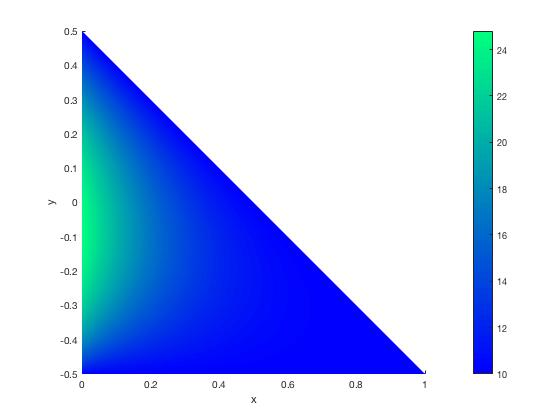
\includegraphics[scale=0.5]{TriangleEDP.jpg}
\end{center}
Voici le script matlab correspondant (Les fonctions seront explicitées ultérieurement) :
\vspace{0.5cm}



% LISTING2 
\begin{lstlisting}[language=Matlab,frame=single,caption=Resolution d'une EDP sur un triangle]
function result = uTriangle(X,area,fc)

model = createpde() ; 
g=triangle(X,area) ; 
% Construit un triangle de cote X et d'aire area
geometryFromEdges(model,g); % geometryFromEdges for 2-D

%Conditions de bord : 
%Les murs non chauffes sont a la temperature exterieure To = 10
applyBoundaryCondition(model,'dirichlet','Edge',[2,3],'u',10);

%Le mur chauffe est modelise par un flux rentrant 
% on suppose que l on a mis un radiateur au niveau du mur 
applyBoundaryCondition(model,'neumann','Edge',[1],'q',0,'g',50);

% Parametres de l'equation
a = 0;
c=1;
a=0;
f=fc;
% On choisit une maille adaptative, car les coins du triangle sont un probleme
[u,p,e,t] = adaptmesh(g,model,c,a,f,'maxt',5000,'par',1e-10);
pdeplot(p,e,t,'XYData',u,'ZData',u,'Mesh','off')
xlabel('x')
ylabel('y')
xlim([-X X])
ylim([-X X])
axis equal
result.u = u ;  % Valeur de u sur chaque mesh
result.p = p ;  % Coordonnees des points 
result.t = t ;
result.e = e ;  % Reference de chacun des points 
end
\end{lstlisting}
\vspace{0.5cm}
Une fois l'équation résolue, il faut maintenant s'interesser à calculer l'intégrale de cette fonction sur le triangle. Pour réaliser cela, nous avons programmé la fonction suivante, qui prend en paramètre la fonction uTriangle ci-dessus, et calcule l'intégrale approchée à l'aide des données fournies par l'algorithme précédent.

\begin{lstlisting}[language=Matlab,frame=single,caption=Calcul de l'integrale]
function I = Integrale(u)

coord = u.p ;    % Contient les coordonnees des sommets 
indices = u.t ;  % Contient les references de chaque element
val = u.u ; 

% On va calculer l integrale en evaluant la valeur de la fonction sur
% chaque petit triangle 
I =0 ; 
area = 0 ; 
for i = 1:length(indices) ;          % Pour chaque triangle 
    a = coord(:,indices(1,i)) ;      % Coord du 1er point 
    b = coord(:,indices(2,i)) ;      % Coord du second point 
    c = coord(:,indices(3,i)) ;      % Coord du troisieme point
    
    moy = (val(indices(1,i))+val(indices(1,i))+val(indices(1,i)))/3 ;
    area = area + 0.5*abs(a(1)*c(2)-a(1)*b(2)+b(1)*a(2)-b(1)*c(2)
    +c(1)*b(2)-c(1)*a(2)) ; 
    I = I + moy*0.5*abs(a(1)*c(2)-a(1)*b(2)+b(1)*a(2)-b(1)*c(2)+c(1)*
    b(2)-c(1)*a(2)) ;
end
    I = I/area ; 
end
\end{lstlisting} 
On peut maintenant mettre en place l'algorithme pour determiner la solution de notre problème. On essaie donc différentes valeurs de $x$ pour une aire fixée à 0.25.
% Script pour trouver le maximum 
% LISTING 3
\begin{lstlisting}[language=Matlab,frame=single,caption=Script Principal]
% Script principal 
x = 0.5:0.01:1.5 ; 
mat = [] ; 
for i = 1:length(x) ;
         mat(i) = Integrale(uTriangle(x(i),1/4,0)) ;
end
plot(x,mat) ; 
xlabel('longueur du cote x')
ylabel('Temperature moyenne')
\end{lstlisting}
\vspace{0.5cm}
Le programme nous retourne la courbe suivante : \\
\begin{center}
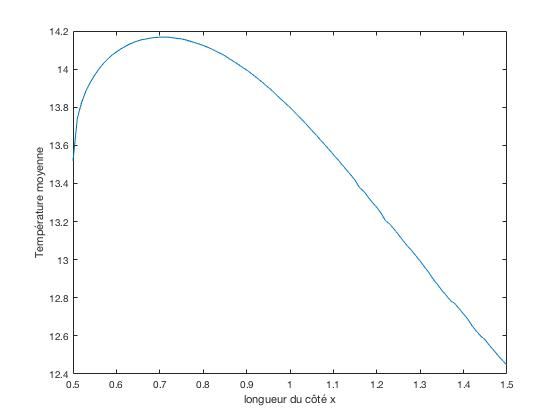
\includegraphics[scale=0.5]{Triangle_CourbeX.jpg}
\end{center}
\newpage

On trouve alors un maximum aux alentours entre $0.70$ et $0.71$ (ce qui ressemble fortement à $\frac{\sqrt{2}}{2}$). Ce n'est pas vraiment une surprise, car on s'attendait à trouver une forme relativement régulière, et dans le cas présent, il s'agit du triangle rectangle équilatéral. \\
\vspace{5cm}
\begin{center}
\begin{picture} (0,0) (20,0) 
\setlength{\unitlength}{2.5cm}
\thicklines
\put(0,0) {\line(0,1) {2}}
\put(0,0) {\line(1,1) {1}}
\put(0,2) {\line(1,-1) {1}}
\put(-0.2,1) {$1$}
\put(0.2,1) {$|\Omega|$}
\end{picture}
\end{center}
\vspace{1cm}
Procédons à quelques remarque. Tout d'abord, on observe que la figure "optimisée" est symétrique, ce qui semble s'accorder avec les conditions aux limites spatiales qui sont elles symétriques par rapport à l'axe des abscisses. Cela explique pourquoi dans la suite de l'étude, nous accorderons une place importante à la symétrie dans les figures recherchées.\\




\newpage
\part{Implémentation d'un premier algorithme sur Python}

\section*{I - Déplacement d'un sommet du polygone avec aire constante}

\pa L'idée général de l'algorithme repose sur le déplacement successif des différents points du polygone et cela en conservant l'aire totale du polygone. Pour cela on va déplacer un sommet sur la droite passant par les deux sommets voisins du sommet. Sur le schéma, nous avons représenté cette droite en rouge. L'idée derrière ce déplacement est d'exploiter la formule sur l'aire d'une triangle : $\mathcal{A} = \frac{\mathcal{B}.h}{2}$ , ou $\mathcal{B}$ est la base du triangle et $h$ est la hauteur du triangle. En déplacant les points de cette façon, nous pouvons conserver la hauteur et la base du triangle considéré par l'algorithme et par conséquent l'aire du triangle. 

\vspace{3.5cm}
\begin{center}
\begin{picture} (100,100) (20,0) 
\setlength{\unitlength}{2.5cm}
\thinlines
\put(0,0) {\color{gray} \line(-2,3) {1}}
\put(-1,1.5) {\color{gray} \line(2,1) {1}}
\thicklines
\put(0,0){\line(-1,1){1}}
\put(-1,1){\line(1,1){1}}
\put(0,0){\line(1,0){2}}
\put(0,-0.5) {\color{red} \line(0,1) {3}}
\put(-1,-0.5) {\color{red} \line(0,1) {3}}
\put(0,2) {\line(1,0) {2}}
\put(2,2) {\line(1,-1) {1}}
\put(2,0) {\line(1,1) {1}}
\put(-1,1) {\vector(0,1) {0.48}}
\put(-1,1.5){\circle*{0.05}}
\put(-1,1){\circle*{0.05}}
\put(-1.2,1.5){$A'$}
\put(-1.2,1){$A$}
\put(0.95,1) {$\Omega$}
\end{picture}
\\
\vspace{1.5cm}
Figure : Déplacement du sommet $A$ selon l'algorithme
\end{center}
\vspace{0.5cm}
\pa L'idée est ensuite de faire varier les différents points du Polygone selon le même schéma de déplacement. Toutefois, la manière de choisir les points à déplacer et les critères d'arrêt sont encore à déterminer.\\

\newpage

\section*{II - Implémentation d'un algorithme sous Python} 
\pa L'idée générale est de créer un objet sous python qui représente un polygone sous Python. Nous avons opté pour la création d'une classe appelée Polygon, qui est constitué d'une liste de points indépendants, qui peuvent être bougés au gré de nos envies. 
\par Présentons succintement les idées générales de l'algorithme que nous avons choisi : \vspace{0.3cm}

\begin{itemize}
  \item On parcourt les sommets du polygone, puis on teste deux petits déplacement de chacun des sommets
  \item On garde en mémoire le déplacement et la valeur de l'intégrale associé à chacun des petits déplacements
  \item Une fois que tous les sommets ont été parcourus, on choisit le meilleur déplacement par rapport à tous les sommets
  \item On applique le déplacement au polygone, puis on recommence 
\end{itemize}
\vspace{0.3cm}
Le calcul de l'intégrale sur le polygone se fait à l'aide de Matlab, qui permet de résoudre directement l'équation differentielle sur le polygone. On a juste à importer la géométrie sous Matlab, puis on utilise la PDE toolbox pour résoudre l'équation différentielle partielle sur nôtre figure. Le seul défaut de cette méthode, est son coût en remaillage, qui prend pas mal de temps. Le temps de calcul de cet algorithme est ainsi assez élevé. 
\par 


\newpage
\section*{III - Résultats de cet algorithme }

\newpage

\pa 





% ///////////////////////////////////////////////////////
%						Partie Annexes
% ///////////////////////////////////////////////////////

\section*{Annexes}


% Classe VECTOR

\begin{lstlisting}[language=Python,frame=single,caption=Création de la classe Vecteur]
class Vector : 
    """ Represente un vecteur """
    
    def __init__(self,x,y) : 
        self.x = x 
        self.y = y 
        
    def __str__(self) : 
        return ("v(%f,%f)" % ( self.x, self.y))
        
        
    # Normalise le vecteur 
    def normalize(self) : 
        norm = (self.x ** 2 + self.y ** 2) ** 0.5
        self.x = self.x / norm 
        self.y = self.y / norm 
\end{lstlisting}

% Classe VERTEX

\begin{lstlisting}[language=Python,frame=single,caption=Création d'une classe Vertex]
class Vertex : 
    """
     La classe Vertex est une classe qui represente les coordonnees des points 
     d'un polygone donne 
    """
    
    def __init__(self, x, y) : 
        
        self.x = x 
        self.y = y 
    
    def __str__(self) : 
        return ("(%f,%f)" % (self.x, self.y) )
    
    def __copy__(self, vertex) : 
        self.x = vertex.x 
        self.y = vertex.y 
    
    #---------------------------------------------------------------------    
    # Deplace le sommet de dx selon x et dy selon y 
    
    def update(self, dx, dy) : 
        self.x += dx 
        self.y += dy 
        
        
    #---------------------------------------------------------------------   
    # deplace le point dans la direction du vecteur unitaire vector 
    
    def move(self, vector, dl) : 
        # On deplace le point selon le vecteur
        dx = dl * vector.x 
        dy = dl * vector.y 
        self.update(dx, dy) 
\end{lstlisting}


% Classe POLYGON

\begin{lstlisting}[language=Python,frame=single,caption=Création de la classe Polygon]
class Polygon : 
    """
        La classe Polygon contient des Vertex (Sommets). L'ensemble de ces 
        sommets forme un polygon 
        
        Les attributs de cette classe sont : 
           _N : le nombre de cotes 
           _vertices : la liste contenant les sommets
    """
    
    def __init__(self, *args) : 
        # Nombre de cotes dans le polygone
        self.N = len(args)                                   
        
        # Liste contenant les sommets (vertex)
        self.vertices = []                                    
        for vertex in args : 
            self.vertices.append(vertex)         
            
            
    # Print
    def __str__(self) : 
        res = "(" 
        for vertex in self.vertices : 
            res = res + vertex.__str__() + ","
        return res[:-1]+')'
    
    #----------------------------------------------------------------------  
    # Retourne les coordonnees x et y d'un sommet 
    #
    # Retourne la coordonnee x du sommet i 
    def getx(self, i) : 
        return self.vertices[i % self.N].x 
    # Retourne la coordonnee y du sommet i 
    def gety(self, i) : 
        return self.vertices[i % self.N].y 
    
    
    #---------------------------------------------------------------------
    # La fonction findCoef renvoie le coefficient directeur de la droite 
    # passant par les sommets i-1 et i+1 
    
    def directorVertice(self, i) : 
        dx = self.getx(i + 1) - self.getx(i - 1)
        dy = self.gety(i + 1) - self.gety(i - 1) 
        res = Vector(dx, dy)
        res.normalize()
        return res 
        
    
    
    #----------------------------------------------------------------------   
    # calcule le vecteur directeur de la droite passant par le cote i 
    def directorSide(self, i) : 
        dy = self.gety(i + 1) - self.gety(i)
        dx = self.getx(i + 1) - self.getx(i)
        res = Vector(dx, dy)
        res.normalize() 
        return res 
          
    



    #---------------------------------------------------------------------    
    # Cette methode construit une geometrie prete a l'exportation sous 
    # matlab
    
    def buildGeometry(self) : 
        # On initialise une liste avec l'argument 2, qui est le code  
        # correspondant a une forme polygonale sous matlab, et self.N est le 
        # nombre de cotes. Cette fonction renvoie une matrice prete a etre  
        # employee dans la fonction Matlab decsg(mat)
        
        mat = [[2], [self.N]] 
        for vertex in self.vertices : 
            mat.append([vertex.x]) 
        for vertex in self.vertices : 
            mat.append([vertex.y]) 
        return mat
        
    #---------------------------------------------------------------------    
    # Deplacement d'un point du polygone selon l'algorithme 
    # i correspond au numero du sommet et dl a la longueur du 
    # deplacement 
    
    def move(self, i, dl) : 
        vector = self.directorVertice(i) 
        self.vertices[i % self.N].move(vector, dl) 
    
        
    #----------------------------------------------------------------------   
    # Calcul de la valeur de l'integrale pour un deplacement du sommet i  
    # d'une longueur dl 
    # La methode ne modifie ainsi pas le polygone lorsque elle est executee 
    
    def valueIntegral(self, i, dl, eng) : 
        self.move(i, dl) 
        mat = matlab.double(self.buildGeometry())
        value = eng.computeIntegral(mat) 
        self.move(i, -dl) 
        return value 
        
    
    
    #----------------------------------------------------------------------   
    # Fonction de tracage 
    
    def plotPY(self) : 
        
        for k in range(self.N) : 
            plt.plot([self.vertices[ k % self.N].x,
                     self.vertices[(k + 1) % self.N].x],
                     [self.vertices[k % self.N].y,
                     self.vertices[(k + 1) % self.N].y],
                     '-r'
                     )
            
        plt.show()
\end{lstlisting}

% MEILLEUR DEPLACEMENT

\begin{lstlisting}[language=Python,frame=single,caption=Trouver le meilleur déplacement]
# On cherche la position du sommet i qui maximise
# la fonctionnelle de forme 

def bestValue(polygon, i, dl, eng) :        
    # On initialise matlab, puis calculons la valeur de l'integrale initiale 
        
    L = np.array([polygon.valueIntegral(i, -dl, eng),             		
    		  # Valeur de l'integrale pour le deplacement a gauche 
                  polygon.valueIntegral(i, 0, eng),               		
                  # Valeur de l'integrale sans deplacement 
                  polygon.valueIntegral(i, dl, eng)])             		
                  # Valeur de l'integrale pour le deplacement a droite 

    index = np.argmax(L)                                          		
    # Retourne l'index du maximum de cette liste
    return [L[index], (index - 1) * dl]               
    
\end{lstlisting}


\begin{lstlisting}[language=Python,frame=single,caption=Boucle principale de l'algorithme]
def oneIteration(polygon, dl, eng) : 
    
    # On cherche le petit deplacement qui maximise notre fonctionnelle 
    # de forme lors d'une iteration de l'algorithme 
    # On examine chacun des sommets independamment
    max = [0,0] 
    rank = 0 
    for i in range(2, polygon.N) : 
        val = bestValue(polygon, i, dl, eng)
        print("val ="+str(val))
        if val[0] > max[0] :
            max = val
            rank = i 
    polygon.move(rank, max[1])   
\end{lstlisting}

\end{document}